\documentclass[twocolumn,numberedappendix]{../aastex62}

% these lines seem necessary for pdflatex to get the paper size right
\pdfpagewidth 8.5in
\pdfpageheight 11.0in

% for the red MarginPars
\usepackage{color}

% some extra math symbols
\usepackage{mathtools}

% allows Greek symbols to be bold
\usepackage{bm}

% allows us to force the location of a figure
\usepackage{float}

% allows comment sections
\usepackage{verbatim}

% Override choices in \autoref
\def\sectionautorefname{Section}
\def\subsectionautorefname{Section}
\def\subsubsectionautorefname{Section}

% MarginPars
\setlength{\marginparwidth}{0.75in}
\newcommand{\MarginPar}[1]{\marginpar{\vskip-\baselineskip\raggedright\tiny\sffamily\hrule\smallskip{\color{red}#1}\par\smallskip\hrule}}

\newcommand{\msolar}{\mathrm{M}_\odot}

% Software names
\newcommand{\amrex}{\texttt{AMReX}}
\newcommand{\boxlib}{\texttt{BoxLib}}
\newcommand{\castro}{\texttt{CASTRO}}
\newcommand{\maestro}{\texttt{Maestro}}
\newcommand{\microphysics}{\texttt{Microphysics}}
\newcommand{\wdmerger}{\texttt{wdmerger}}
\newcommand{\python}{\texttt{Python}}
\newcommand{\matplotlib}{\texttt{matplotlib}}
\newcommand{\yt}{\texttt{yt}}
\newcommand{\vode}{\texttt{VODE}}
\newcommand{\isoseven}{\texttt{iso7}}
\newcommand{\aproxthirteen}{\texttt{aprox13}}
\newcommand{\aproxnineteen}{\texttt{aprox19}}
\newcommand{\aproxtwentyone}{\texttt{aprox21}}

\begin{document}

%==========================================================================
% Title
%==========================================================================
\title{Numerical Stability of Detonations in White Dwarf Simulations}

\shorttitle{Numerical Detonations}
\shortauthors{Katz et al. (2018)}

\author{Max P. Katz}
\affiliation
{
  NVIDIA Corporation, 2788 San Tomas Expressway, Santa Clara, CA, 95051, USA
}

\author{Michael Zingale}
\affiliation
{
  Department of Physics and Astronomy, Stony Brook University, Stony Brook, NY, 11794-3800, USA
}



%==========================================================================
% Abstract
%==========================================================================
\begin{abstract}
Some simulations of Type Ia supernovae feature thermonuclear detonations that
arise self-consistently during the evolution. It is not clear whether these
detonations would occur in a simulation that fully resolved the burning. In this
study we examine a test detonation problem inspired by collisions of white dwarfs.
This test problem demonstrates that achieving a converged thermonuclear ignition
requires spatial resolution finer than 1 km in the burning region, and that
the simulation as a whole likely needs a base resolution on the order of 1 km.
Current computational resource constraints place this stringent resolution requirement
out of reach for almost all multi-dimensional supernova simulations.
Consequently, contemporary simulations that self-consistently demonstrate
detonations are very likely not resolved and should not be trusted.
\end{abstract}
\keywords{supernovae: general - white dwarfs}

%==========================================================================
% Introduction
%==========================================================================
\section{Introduction}
\label{sec:introduction}

Thermonuclear detonations are common to all current likely models of Type Ia
supernovae (SNe Ia), but how they are actually generated in progenitor systems
is still an open question. Different models predict different locations for
the detonation and different mechanisms for initiating the event. Common to all
of the cases is a severe lack of numerical resolution in the location where the
detonation is expected to occur. The length and time scale at which a detonation
forms is orders of magnitude smaller than the resolution that typical multi-dimensional
hydrodynamic simulations can achieve. The mere presence of a detonation (or lack thereof)
in a simulation is therefore only weak evidence regarding whether a detonation would truly occur.

In this study we examine the challenges associated with simulating thermonuclear detonations.
The inspiration for this work comes from the literature on head-on collisions of WDs,
which can occur, for example, in certain triple star systems \citep{thompson:2011,hamers:2013}.
WD collisions rapidly convert a significant amount of kinetic energy into thermal energy and
thus set up conditions ripe for a thermonuclear detonation. Collisions are interesting
from the simulation perspective because of both this susceptibility to detonation and
the relative ease in setting them up.

Early studies on WD collisions \citep{rosswog:2009,raskin:2010,loren-aguilar:2010,
hawley:2012,garcia-senz:2013} typically had effective spatial resolutions in the
range 100--500 km, and observed detonations that convert a large amount of
carbon/oxygen material into iron-group elements. These studies varied in methodology
(Lagrangian versus Eulerian evolution, nuclear network used) and did not closely agree
on the final result of the event (see Table 4 of \cite{garcia-senz:2013} for a summary).
\cite{kushnir:2013} argued that many of these simulations featured numerically unstable
evolution, ultimately caused by the zone size being significantly larger than the length
scale over which detonations form. The detonation length scale can vary widely based
on physical conditions \citep{seitenzahl:2009,garg:2017} but is generally much
smaller than 100 km. In this paper, we attempt to find what simulation length scale
is required to achieve converged thermonuclear ignitions.



%==========================================================================
% 1D collision test problem
%==========================================================================
\section{Test Problem}
\label{sec:collisions}

Our test problem is inspired by \cite{kushnir:2013}, and very loosely approximates the
conditions of two $0.64\ \msolar$ WDs colliding head-on. The simulation domain is 1D with a
reflecting boundary at $x = 0$. For $x > 0$ there is a uniform fluid composed (by mass)
of $50\%\, ^{12}$C, $45\%\, ^{16}$O, and $5\%\, ^{4}$He. The fluid is relatively cold,
$T = 10^7$ K, has density $\rho = 5 \times 10^6$ g/cm$^3$, and is traveling toward the
origin with velocity $-2 \times 10^8$ m/s. A uniform constant gravitational acceleration
is applied, $g = -1.1 \times 10^8$ m/s$^{2}$. This setup causes a sharp initial release
of energy at $x = 0$, and the primary question is whether a detonation occurs promptly
near this contact point, or occurs later (possibly at a distance from the contact point).
The simulated domain has width $1.6384 \times 10^9$ cm, and we apply inflow boundary conditions
that keep feeding the domain with material that has the same conditions as the initial fluid.
Simulations are performed with the adaptive mesh refinement (AMR) code \castro\
\citep{castro, astronum:2017}. For the burning we use the alpha-chain nuclear network
\texttt{aprox13}. The results we describe below do not strongly depend on the network.

The simulation is terminated when the peak temperature on the domain first reaches
$4 \times 10^9$ K, which we call a thermonuclear ignition. This stopping criterion is a
proxy for the beginning of a detonation. Reaching this temperature does not guarantee
that a detonation will begin, and in this study we do not directly address the question
of whether a ignition of this kind always leads to a detonation. Rather, the main question
we investigate here is whether this ignition is numerically converged. A converged ignition
is a prerequisite to having a converged detonation. We measure two diagnostic quantities:
the time since the beginning of the simulation required to reach this ignition criterion,
and the distance from the contact point of the peak temperature.

The only parameter we vary in this study is the spatial resolution used for this problem.
We vary both the base resolution of the grid, and also the amount of refinement allowed.
AMR is applied on gradients of the temperature: we tag zones for refinement if the temperature
varies by more than 50\% between two zones. Timesteps are limited only by the hydrodynamic
stability constraint, with CFL number 0.5. Although this leads to Strang splitting error
in the coupling of the burning and hydrodynamics for low resolution, we have verified that
the incorrect results seen at low resolution do not meaningfully depend on the timestep constraint
(both by applying a timestep limiter based on nuclear burning, and by using the spectral deferred
corrections driver in \castro, which directly couples the burning and hydrodynamics). At very high
resolution, the splitting error automatically becomes unimportant as the CFL criterion decreases
the timestep.

\begin{figure}[ht]
  \centering
  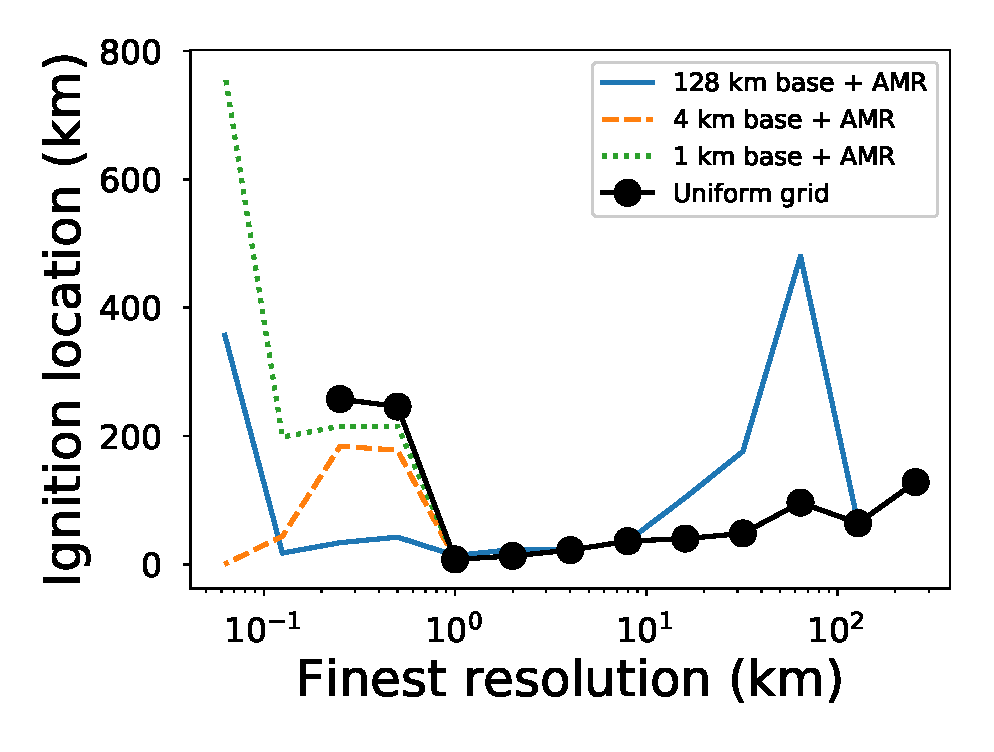
\includegraphics[scale=0.525]{{{plots/amr_ignition_self-heat}}}
  \caption{Distance from the contact point of the ignition as a function of finest
           spatial resolution. The solid black curve with circle markers represents
           the simulations with uniform resolution (no AMR). The other curves represent
           simulations with a fixed base resolution and varying amounts of AMR.
           \label{fig:self-heat-distance}}
\end{figure}

\autoref{fig:self-heat-distance} shows our main results. The lowest resolution we consider,
256 km, is typical of the early simulations of white dwarf collisions, and demonstrates a
prompt ignition near the contact point. As the (uniform) resolution increases, the ignition
tends to occur earlier and nearer to the contact point. This trend is not physically meaningful:
all simulations with resolution worse than about 1 km represent the same prompt central ignition,
and as the resolution increases, there are grid points physically closer to the center that can ignite.
However, when the resolution is better than 1 km, the situation changes dramatically: the prompt
central ignition does not occur, but rather the ignition is delayed and occurs further from the contact
point. When we have finally converged, the ignition occurs around 1000 km from the contact point,
about 1 second after contact (contrast to less than 0.05 seconds for the simulation with 1 km resolution).
This story contains two important lessons. First, the required resolution for a converged simulation,
less than 100 m, is out of reach of current 3D supernova simulations. Second, the behavior for
resolutions worse than 1 km qualitatively appears to be converged, and one could perhaps
be misled into thinking that there was no reason to try higher resolutions, which is reason
for caution in interpreting reacting hydrodynamics simulations.

Also in \autoref{fig:self-heat-distance} we show results for a few cases where we add AMR
using the criterion described above. The main takeaway here is that for coarse grid resolutions
worse than 1 km, the addition of AMR yields unreliable results: the coarse grid's approximation
of the physics must simply not be good enough for refinement to do any good. This parallels the
fact that the trend of convergence towards the correct delayed detonation does not begin until
resolutions better than 1 km. However, for a coarse grid resolution of 1 km, AMR does yield
convergence to the correct answer, and at a much cheaper computational cost than the equivalent
uniform grid simulation\marginpar{quantify this}, so AMR does add value if the resolution on the
coarse grid is sufficiently high.



\section{Numerically Unstable Burning}
\label{sec:unstable_burning}

\citet{kushnir:2013} observe an important possible failure mode
for reacting hydrodynamics simulations. Let us define $\tau_e = e / \dot{e}$
as the nuclear energy injection timescale, and $\tau_s = \Delta x / c_s$
as the sound-crossing time in a zone (where $\Delta x$ is the grid
resolution and $c_s$ is the speed of sound).
When the sound-crossing time is too long, energy is built up in
a zone faster than it can be advected away by pressure waves.
This is of course a problem inherent only to numerically discretized
systems as the underlying fluid equations are continuous.
This can lead to a numerically seeded detonation caused by the
temperature building up too quickly in the zone; the detonation
may be spurious in this case. If $\tau_s \ll \tau_e$, we can be
confident that a numerically seeded detonation has not occurred.
In practice, we will quantify this as:
\begin{equation}
  \tau_s \leq f_{s}\, \tau_e \label{eq:burning_limiter_2}
\end{equation}
and require that $f_{s}$ is sufficiently smaller than one.
\citet{kushnir:2013} state that $f_{s} = 0.1$ is a sufficient
criterion. \citet{kushnir:2013} enforced this criterion on
their simulations by artificially limiting the magnitude of the energy
release after a burn.

To understand this choice, consider the outcome of our baseline case.
When the two WDs collide, there is a prompt detonation
at the contact point at the center of the domain. This detonation occurs
when the density is relatively low because the WDs have not had much
time to collide, and so the nucleosynthetic yield of nickel is low. If
this is the case, the colliding WDs are not a good candidate for
normal SNe Ia. However, if this detonation is delayed, material builds
up at a stalled shock in the center, and the eventual detonation occurs
on the outer edge of the stalled shock. There will then be much more
high density material to process into nickel, and the resulting
explosion creates an amount of nickel potentially sufficient to explain
normal SNe Ia. The discussion thus centers on whether the prompt detonation
is physical. \citeauthor{kushnir:2013} argues that it is not, on the basis
that $\tau_s > \tau_e$ when this detonation occurs. We find the same thing:
for the baseline case, the sound-crossing time is about five times longer
than the energy injection time. This means that an ignition is guaranteed
to occur for numerical reasons. \citeauthor{kushnir:2013} thus argue that
the suppressed burn is justifiable, as it suppresses this prompt detonation.

This argument is flawed because a physical detonation may \textit{also}
occur this way. For example, consider a region of WD material at uniformly
high temperature, say $5 \times 10^9\ \text{K}$, with an arbitrarily large size,
say a cube with side length 100 km. This region will very likely ignite,
even if it is surrounded by much cooler material. By the time the material on
the edges can advect heat away, the material in the center will have long since
started burning carbon, as the sound crossing time scale is sufficiently large
compared to the energy injection time scale. This is true regardless of whether
the size of this cube corresponds to the spatial resolution in a simulation.
Suppression of the burn in this case is unphysical: if we have a zone matching
these characteristics, the zone should detonate.

When the resolution is low enough, there is a floor on the size of a hotspot,
possibly making such a detonation more likely. This is an unavoidable consequence
of the low resolution; yet, it may be the correct result of the simulation that
was performed. That is, even if large hotspots are unphysical because in reality
the temperature distribution would be smoother, if such a large hotspot \textit{were}
to develop (which is the implicit assumption of a low resolution simulation), then
it would likely detonate. If the results do not match what occurs at higher
resolution, then the simulation is not converged and the results are not reliable.
However, it may also be the case that a higher resolution simulation will yield
similar results, for example because even at the higher resolution, the physical
size of the hotspot stays the same. Additionally, one might think that simply
adding adaptive mesh refinement in the burning region could help, because then
$\Delta x$ decreases, so the ratio of $\tau_s$ to $\tau_e$ should decrease.
We developed an AMR criterion to do just this: we tag on regions suggested by
the burning stability criterion, \autoref{eq:burning_limiter_2}. But if a low
resolution simulation develops a very large hotspot that violates the stability
criterion, adding refinement inside this region will likely not help, because the
energy trapped in the center of the region may not be able to escape before ignition
occurs. So for the simulations with resolution inside the stars that was coarser than
10 km, even adding a significant amount of refinement (say, refining by a factor of
64 or 128) did not change the propagation of a detonation.

For the above reasons, an appeal to the numerical instability criterion alone is
insufficient to understand whether a given ignition is real. We find that \textit{all}
of the detonations we have seen at any resolution violate the stability criterion,
even for the finest resolution simulation we performed (150 m, inside the burning region).
This is true even if the prompt detonation is suppressed:
the delayed detonation also is numerically unstable. For comparison purposes, we
developed an option for our burner to use a ``suppressed'' burning mode. In a
suppressed burn, we limit the changes to the state so that \autoref{eq:burning_limiter_2}
is always satisfied\footnote{To achieve this we directly multiply the
right-hand-side vector in the integration by a factor $F$
for all variables, where $F$ is the multiplicative factor needed to
be applied to $\dot{e}$ such that the equality in \autoref{eq:burning_limiter_2}
holds. (If the inequality is already satisfied, then the integration
vector is not modified.) We fix $\tau_s$ to be the value of the sound
crossing time at the beginning of the burn (that is, we do not
update it as the sound speed changes) and we fix the energy $e$
that goes into the estimate for $\tau_e$ to be the value of the
internal energy of the zone at the beginning of the burn.}. When we
evolve the baseline case with this suppressed burner, the prompt detonation
is indeed suppressed. A later detonation does occur, but this delayed
detonation also triggers the suppression. The result is that the detonation
does not get to very high temperatures, and the result is again a ``failed''
supernova that does not generate nearly enough nickel. Thus we do not
reproduce the claim of \citeauthor{kushnir:2013} that the suppressed
burning mode suppresses only the prompt detonation, but allows the
delayed detonation to occur. We could find some way to turn off the
suppression and allow the delayed detonation, but without some independent
confirmation that the delayed detonation is physical (while the prompt
detonation is not) this would be begging the question.

The upshot of this discussion is that the only way to resolve the
question is with higher resolution simulations. The semi-analytic
criterion provided by \cite{garg:2017}, and the numerical calculations
of \cite{seitenzahl:2009}, give critical radii for spontaneous detonation.
For the densities we are interested in ($\sim 10^7\ \text{g\,/\,cm}^3$),
assuming equal C/O material, the critical radii are in the range 1-10 km.
So this suggests that our simulation needs to do significantly better than
this if we are likely to make headway on this issue. Detonations observed
at higher resolution may be physically plausible because the critical
temperature gradient can be resolved. The high resolution needs to be
achieved with some combination of high resolution of the collision process
itself, and AMR based on the stability criterion as described
above, where we tag for refinement all zones above some $f_{s}$, the
ratio of the sound crossing time to the energy injection time. We
cannot solely rely on a low resolution run with AMR based on the
burning stability criterion for the reason described above, that a
detonation may be spuriously locked in by the low resolution regardless
of how much resolution we can practicably add to it.



%==========================================================================
% Conclusions
%==========================================================================
\section{Conclusions and Discussion}\label{Sec:Conclusions and Discussion}
\label{sec:conclusion}

% Add discussion about how none of the conclusions depend on the microphysics
% of how ignitions/detonations actually occur -- this paper is simply about
% self-consistent fluid simulations, i.e. are we even correctly solving
% the equations we wrote down, and not focusing on the harder question
% of whether we're solving the right equations.


\acknowledgments

This research was supported by NSF award AST-1211563 and DOE/Office of
Nuclear Physics grant DE-FG02-87ER40317 to Stony Brook. An award of
computer time was provided by the Innovative and Novel Computational
Impact on Theory and Experiment (INCITE) program.  This research used
resources of the Oak Ridge Leadership Computing Facility located in
the Oak Ridge National Laboratory, which is supported by the Office of
Science of the Department of Energy under Contract
DE-AC05-00OR22725. Project AST106 supported use of the ORNL/Titan
resource.  This research used resources of the National Energy
Research Scientific Computing Center, which is supported by the Office
of Science of the U.S. Department of Energy under Contract
No. DE-AC02-05CH11231. The authors would like to thank Stony Brook
Research Computing and Cyberinfrastructure, and the Institute for
Advanced Computational Science at Stony Brook University for access
to the high-performance LIred and SeaWulf computing systems, the latter
of which was made possible by a \$1.4M National Science Foundation grant (\#1531492).

The authors thank Chris Malone and Don Willcox for useful discussions
on the nature of explosive burning, and Doron Kushnir for providing
clarification on the nature of the burning limiter used in \cite{kushnir:2013}.

This research has made use of NASA's Astrophysics Data System 
Bibliographic Services.

\clearpage

\bibliographystyle{../aasjournal}
\bibliography{../refs}

\end{document}
